\documentclass[a4paper,UTF8]{article}
\usepackage{ctex}
\usepackage[margin=1.25in]{geometry}
\usepackage{color}
\usepackage{graphicx}
\usepackage{amssymb}
\usepackage{amsmath}
\usepackage{amsthm}
%\usepackage[thmmarks, amsmath, thref]{ntheorem}
\theoremstyle{definition}
\newtheorem*{solution}{Solution}
\newtheorem*{prove}{Proof}
\usepackage{multirow}
\usepackage{url}
\usepackage[colorlinks,urlcolor=blue]{hyperref}
\usepackage{enumerate}
%\usepackage{cite}
\renewcommand\refname{参考文献}
\graphicspath{{picforrepo/}{logo/}}
%--

%--
\begin{document}
\title{\textbf{《计算机图形学》十月报告}}
\author{181860127   姚逸斐  \href{mailto:181860127@smail.nju.edu.cn}{181860127@smail.nju.edu.cn}}
\maketitle

\section{综述}
九月里我学习了生成直线的DDA算法、Bresenham算法;生成椭圆的中点圆生成算法;以及生成曲线的Bezier算法和B-spline算法。
并且在cg\_algorithms.py中实现了部分相应算法。

十月里我将生成椭圆的中点圆生成算法以及部分图元的编辑算法运用到实践中,并学习了'Cohen-Sutherland'和'Liang-Barsky'线段裁剪算法并尝试运用到实践中。

十一月里我完成了cg\_cli.py中大部分指令的实现,并通过编写一些测试用例调试后对之前cg\_algorithms.py中的一些bug进行了修复。

\section{算法介绍}
\subsection{直线}

\subsubsection{DDA算法}
\textbf{原理介绍}\par
DDA算法的主要思想是由直线公式$y = kx + b$推导出来的。
我们已知直线段两个端点$P_0(x_0,y_0)$和$P_1(x_1,y_1)$,就能求出 k 和 b 。
在k,b均求出的条件下,只要知道一个x值,我们就能计算出一个y值。如果x的步进为1(x每次加1,即$x = x +1$),那么y的步进就为$k+b$;同样知道一个y值也能计算出x值,此时y的步进为1,x的步进为$\frac{(1-b)}{k}$。
根据计算出的x值和y值,向下取整,得到坐标$(x',y')$,并在$(x',y')$处绘制直线段上的一点。

为进一步简化计算,通常可令b取0,将起点看作$(0,0)$。设当前点为$(x_i, y_i)$则用DDA算法求解$(x_i+1,y_i+1)$的计算公式可以概括为:
\begin{align}
    x_i+1 = x_i + xStep \\
    y_i+1 = y_i + yStep 
\end{align}

我们一般通过计算 $Δx$ 和 $Δy$ 来确定$xStep$和$yStep$:

如果 $Δx > Δy$ ,说明x轴的最大差值大于y轴的最大差值,x轴方向为步进的主方向,$xStep = 1$,$yStep = k$;
如果 $Δy> Δx$,说明y轴的最大差值大于x轴的最大差值,y轴方向为步进的主方向,$yStep = 1$,$xStep = \frac{1}{k}$。
根据这个公式,就能通过$(x_i , y_i)$迭代计算出$(x_{i+1} , y_{i+1})$,然后在坐标系中绘制计算出的$(x,y)$坐标点。\cite{DDA}


\textbf{个人理解\&对比分析}\par
DDA算法依据斜率的绝对值是否大于一分为两种情况,绝对值小于一时,x和y方向的增量值分别为1和k;否则增量值分别为$\frac{1}{k}$和$1$。
$x=a$这种情况,无法计算k值,作为特殊情况处理,$x$不变,$y$迭代加一。



\subsubsection{Bresenham算法}
\textbf{原理介绍}\par
对于直线$y=mx + b$ (我们这里假定$0\leq m \leq 1$,而且两个顶点满足 $x_0 < x_1$ 且 $y_0 < y_1$ ,后面会讨论一般的情况)来说,我们在取样位置 $x_k+1$处,有$y = m( x_k +1) + b$,其中 $d_{lower}$ 和 $d_{upper}$ 分别标识两个像素点与y之间的偏移量,
因此可以得到如下的关系:
\begin{align}
d_{lower} &=y-y_k \\
&= m(x_k+1)+b-y_k \\
d_{upper} &=(y_k+1)-y \\
&=y_k+1-m(x_k+1)-b
\end{align}
我们通过对$d_{lower}$ 和 $d_{upper}$做差可以确定哪个像素更接近y:
\begin{align}
d_{lower}-d_{upper}=2m(x_k+1)-2y_k+2b-1
\end{align}
我们通过对上面的式子进行重新安排来获得画线算法第k步的\textbf{决策参数}$p_k$,从而可以仅使用整数来进行计算。设 $\Delta y$ 和 $\Delta x$ 
分别表示两个顶点垂直和水平的偏移量,令 $m=\frac{\Delta y}{\Delta x}$ ,
我们可以将决策参数定义为:
\begin{align}
p_k &=\Delta x(d_{lower}-d_{upper})b \\
&= 2\Delta y*x_k-2\Delta x*y_k+c
\end{align}
这里 $p_k$ 的符号与$(d_{lower}-d_{upper})$符号相同(基于上面的假定 $\Delta x>0$),参数c是常量,
其值为 $2\Delta y+\Delta x(2b-1)$ ,与像素的位置无关。
当$d_{lower}-d_{upper}$ (即 $p_k<0$)时,
我们认为 $y_k+1$ 处的像素更加接近于线段,也就是我们这里可以通过 $p_k$ 的值来决策出 
$x_{k+1}$处y的值。为了决策出 $x_{k+2}$ 处的值我们需要算出 $p_{k+1}$ :
\begin{align}
p_{k+1} &= 2\Delta y*x_{k+1}-2\Delta x*y_{k+1}+c \\
p_{k+1}-p_k &= 2\Delta y*(x_{k+1}-x_k)-2\Delta x*(y_{k+1}-y_k)
\end{align}
基于我们之前的假定,我们这里x的值会不断增加,
有 $x_{k+1}=x_k+1$,因此:
\begin{align}
    p_{k+1}=p{k}+2\Delta y-2\Delta x(y_{k+1}-y_k)
\end{align}
由于我们之前已经得到了$p_k$的值,
而且知道了$y_{k+1}-y_k$的值为0或1(取决于$p_k$ 的符号)。

该决策过程的递推开始于线段的起点 $(x_0,y_0)$ ,此时的 $p_0$ 可以通过上面的式子得到:
(利用$y = mx + b$ 和 $m=\frac{\Delta y}{\Delta x}$代入化简)
\begin{align}
p_0=2\Delta y-\Delta x
\end{align}
当斜率绝对值 $|m|$小于1时,
我们可以得到Bresenham算法的计算步骤(如图1所示):\par
\begin{figure}[ht]

    \centering
    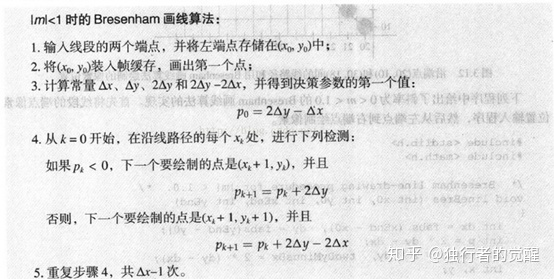
\includegraphics[width = .8\textwidth]{alg.jpg}
    \caption{计算步骤}
    \label{fig:label1}
\end{figure}

\begin{figure}

    \centering
    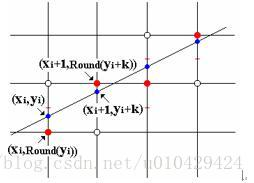
\includegraphics{20170904103100016.jpg}
    \caption{Bresenham算法直线绘制示意图}
    \label{fig:label2}
\end{figure}
\par   

我们上面讨论的直线$y = mx + b$是基于
$0\leq m\leq 1$以及$x_0<x_1$且 $y_0 < y_1$ 
假定的,
也就是说要求 $\Delta y \leq \Delta x$ 而且直线的绘制顺序是从左上到右下的,我们可以拓展此算法:

1)使之可以绘制任何的直线。第一个扩展是绘制反方向,即从右下到左上,这可以在$x_0 > x_1$的情况下简单的交换起点和终点来做到;

2)绘制斜率为负数的情况。可以通过检查$y_0\geq y_1$ 满足的情况下改变y的更新方式,
将$y+1$变为$y-1$来满足这种情况;

3)绘制斜率大于1的情况。我们只需要对$y = mx + b$做关于 $y=x$的映射,即交换计算过程中的x和y来满足这种情况,
并在plot参数时交换参数顺序。   
\cite{Bresenham}

\textbf{个人理解}\par
当斜率绝对值小于一时,x每次加一,以每一小格的中点为界,如果对应的y在中点下方,则取前一个y值,如果对应的y在中点上方,则取前一个y值加一。斜率绝对值大于一时,将x,y对调。


\subsubsection{对比分析}\par
两种算法的运行结果情况如图3所示,从图中可已看出,两种算法都能绘制出直线段,但是在细节稍有不同,
当x=4时,DDA算法的y值为3,而Bresenham的算法y为2。在不过从效率上看,由于Bresenham避免了浮点运算,所以效率更高。\cite{DDA}
\begin{figure}[h]

    \centering
    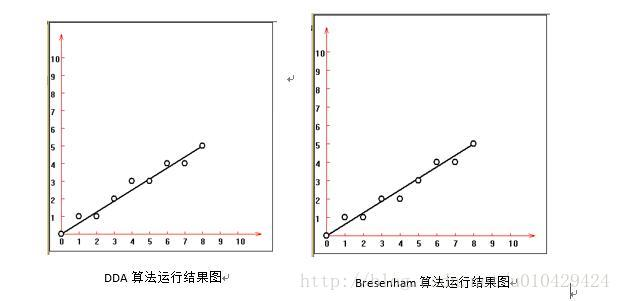
\includegraphics[width = .8\textwidth]{cmp.jpg}
    \caption{DDA与Bresenham算法对比分析}
    \label{fig:label3}
\end{figure}
\par   

\subsection{多边形}
多边形实际上是由多条线段连接而成的,
那么采用线段生成算法(DDA或Bresenham)生成各个线段即可。
\subsection{椭圆}
\subsubsection{中点圆生成算法}
\textbf{原理介绍}\par
椭圆方程:$F(x,y)=b^2x^2+a^2y^2-a^2b^2=0$

定义椭圆弧上某点的切线法向量N如下:
\begin{align}
N(x,y) &= \frac{\partial F(x,y)}{\partial x}i + \frac{\partial F(x,y)}{\partial y}j \\
& = 2b^2xi+2a^2yj
\end{align}
 对方程分别求x偏导和y偏导,最后得到椭圆弧上$(x,y)$
点处的法向量是$(2b^2x,2a^2y)$。椭圆弧法向量的y分量比较大,
即:$2b^2(x+1)<2a^2(y–0.5)$;椭圆弧法向量的x分量比较大,即:
$2b^2(x+1)>2a^2(y–0.5)$。
 
y方向每变化1个单位,x方向变化大于一个单位,因此中点算法需要沿着x方向步进画点,x每次增量加1,求y的值。
同理,中点算法沿着y方向反向步进,y每次减1,求x的值。
 
假设当前位置是$P(x_i,y_i)$,则下一个可能的点就是P
点右边的$P_1(x_i+1,y_i)$点或右下方的$P_2(x_i+1,y_i-1)$
点,取舍的方法取决于判别式$d_i$:
\begin{align}
d_i=F(x_i+1,y_i-0.5)=b^2{(x_i+1)}^2+a^2{(y_i-0.5)}^2–a^2b^2
\end{align}
若$d_i<0$,表示像素点P1和P2的中点在椭圆内,这时可取
P1为下一个像素点。此时$x_{i+1}=x_i+1,y_{i+1}=y_i,d_{i+1}=d_i+b^2(2x_i+3)$

计算出$d_i$的增量是$b^2(2x_i+3)$。

同理,若$di\geq0$,表示像素点P1和P2的中点在椭圆外,
这时应当取P2为下一个像素点。
此时
\begin{align}
x_{i+1}=x_i+1,y_{i+1}=y_i-1,\\
d_{i+1}=d_i+b^2(2x_i+3)+a^2(-2y_i+2)
\end{align}

计算出$d_i$的增量是$b^2(2x_i+3)+a^2(-2y_i+2)$。
计算$d_i$的增量的目的是减少计算量,提高算法效率,
每次判断一个点时,不必完整的计算判别式$d_i$,
只需在上一次计算出的判别式上增加一个增量即可。
\cite{Circle}


%\textbf{个人理解}\par

%\textbf{对比分析}\par
\subsection{曲线}
\subsubsection{Bezier算法}
\textbf{原理介绍}\par
贝塞尔曲线于1962年,由法国工程师皮埃尔·贝塞尔(Pierre Bézier)所广泛发表,他运用贝塞尔曲线来为汽车的主体进行设计。贝塞尔曲线最初由 Paul de Casteljau 于1959年运用 de Casteljau 算法开发,以稳定数值的方法求出贝塞尔曲线。
给定点 P0、P1,线性贝塞尔曲线只是一条两点之间的直线。这条线由下式给出:
\begin{align}
B(t)=P_0+(P_1-P_0)t=(1-t)P_0+tP_1,t\in[0,1]
\end{align}
且其等同于线性插值。

二次方贝塞尔曲线的路径由给定点
$P0、P1、P2$ 的函数 B(t) 追踪:
\begin{align}
B(t)=(1-t)^{2}P_0+2t(1-t)P_1+t^{2}{P}_2,t\in[0,1]
\end{align}
TrueType 字型就运用了以贝塞尔样条组成的二次贝塞尔曲线。
\begin{figure}[ht]
    \centering
    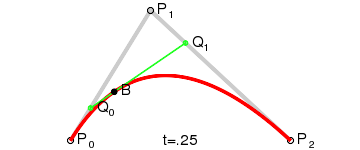
\includegraphics[width = .8\textwidth]{Bezier_2.png}
    \caption{二次Bezier曲线的结构}
    \label{fig:label4}
\end{figure}

$P_0、P_1、P_2、P_3$ 四个点在平面或在三维空间中定义了三次方贝塞尔曲线。
曲线起始于 $P_0$ 走向 $P_1$,并从 $P_2$ 的方向来到 $P_3$。
一般不会经过 $P_1$ 或 $P_2$;这两个点只是在那里提供方向资讯。
$P_0$ 和 $P_1$ 之间的间距,决定了曲线在转而趋进 $P_3$ 之前,
走向 $P_2$ 方向的“长度有多长”。

曲线的参数形式为:
\begin{align}
B(t)=P_0{(1-t)}^3+3P_1t{(1-t)}^2+3P_2t^2{(1-t)}+P_3t^3,t\in[0,1]
\end{align}
现代的成象系统,如 PostScript、Asymptote 和 Metafont,运用了以贝塞尔样条组成的三次贝塞尔曲线,用来描绘曲线轮廓。\cite{Bezier}
\begin{figure}[ht]
    \centering
    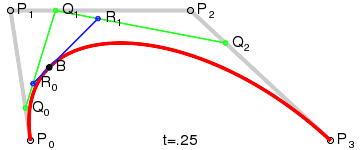
\includegraphics[width = .8\textwidth]{Bezier_3.png}
    \caption{三次Bezier曲线的结构}
    \label{fig:label5}
\end{figure}

%对于$P_0,P_1,…,P_n$,其贝塞尔曲线即:
%\begin{align}
%B(t)=\Sigma_{i=0}^n\tbinom{n}{i}P_i{(1-t)}^{n-i}t^i=P_0(1-t)^n+\tbinom{n}{1}P_1{(1-t)}^{n-1}t+...+P_nt^n,t\in[0,1]
%\end{align}

%\textbf{个人理解}\par

%\textbf{对比分析}\par
\subsubsection{B-spline算法}
\textbf{原理介绍}\par
B-样条曲线,是B-样条基函数的线性组合,是贝塞尔曲线的一般化。
给定n+1个控制点,P0,P1, ..., Pn以及一个节点向量$U={u_0,u_1, ...,u_m}$, p 次B-样条曲线由这些控制点和节点向量U 定义,其公式为:
\begin{align}
C(u)=\Sigma_{i=0}^nN_{i,p}(u)P_i
\end{align}
在上式中,$N_{i,p}(u)$是p次B-样条基函数。

\textbf{节点向量:}设U是m + 1个非递减数的集合,
$u_0\leq u_1\leq u_2\leq...\leq u_m$。
$u_i$称为节点(knots), 集合U称为节点向量(knot vector),
半开区间$[u_i, u_{i+1})$ 是第i个节点区间(knot span)。
注意某些$u_i$可能相等,某些节点区间会不存在。
如果一个节点$u_i$出现 k 次 (即,$u_i=u_{i+1}=...=u_{i+k-1}$),
其中 k > 1, $u_i$是一个重复度(multiplicity)为k 的多重节点,写为 $u_i(k)$。
否则,如果$u_i$只出现一次,它是一个简单节点。如果节点等间距(即, $u_{i+1}-u_i$ 是一个常数,
对 $0\leq i\leq m-1$),节点向量或节点序列称为均匀的;
否则它是非均匀的。一般情况下,我们经常使用 $u_0=0$和 $u_m=1$,
所以定义域是闭区间[0,1]。

\textbf{基函数定义:}为了定义B-样条基函数,我们还需要一个参数,基函数的次数(degree)p,第i个p次B-样条基函数,
写为$N_{i,p}(u)$,递归定义如下:
$$ N_{i,0}(u)=\left\{
\begin{array}{rcl}
1       &      & {if u_i\leq u\leq u_{i+1}}\\
0     &      & {otherwise}
\end{array} \right. $$
\begin{align}
N_{i,p}(u)=\frac{u-u_i}{u_{i+p}-u_i}N_{i,p-1}(u)+\frac{u_{i+p+1}-u}{u_{i+p+1}-u_{i+1}}N_{i+1,p-1}(u)
\end{align}
上述公式通常称为Cox-de Boor递归公式。\cite{B-spline}
%\textbf{个人理解}\par
\subsection{平移变换}
\textbf{原理介绍}\par
平移是指将物体沿直线路径从一个坐标位置移动到另一个坐标位置的变换,如下图所示。
\begin{figure}[h]

    \centering
    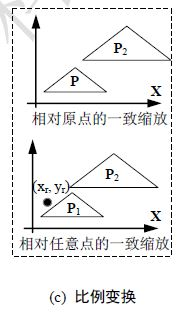
\includegraphics[width = .2\textwidth]{zoom.JPG}
    \caption{平移}
    \label{fig:label6}
\end{figure}
平移变换不改变图形的大小和形状,物体上的每个点移动相同的偏移量,是
一种不产生变形而移动物体的刚体变换。
给定xy平面上的一个点$P_1(x_1,y_1)$,加上平移距
离$T(t_x,t_y)$后得到新的点$P_2(x_2,y_2)$ ,
$t_x$为沿X方向的平移量,$t_y$为沿Y方向的平移量,则
有:
\begin{equation}
    \left\{
                 \begin{array}{lr}
                 x_2 = x_1 + t_x\\
                 y_2 = y_1 + t_y 
                 \end{array}
    \right.
\end{equation}

平移变换的向量表示为:
$P_2 = P_1 + T$ ,其中:
\begin{align}
P_1 =  \begin{bmatrix} x_1&y_1  \end{bmatrix}, P_2 =  \begin{bmatrix} x_2& y_2  \end{bmatrix},
T =  \begin{bmatrix} t_x&t_y  \end{bmatrix}
\end{align}

平移变换的齐次表示为:
\begin{align}
    \begin{bmatrix} x_2 & y_2& 1  \end{bmatrix} = \begin{bmatrix} x_1& y_1& 1  \end{bmatrix}
    \begin{bmatrix} 
        1 & 0 & 0 \\
        0 & 1 & 0 \\ 
        t_x & t_y & 1 
    \end{bmatrix}
\end{align}


直线的平移是将平移向量施加到直线的每个端点;多边形的平移是将平移向量施加
到多边形的每个顶点;曲线可用同样方法来平移:为了改变圆或椭圆的位置,可以平移
其中心坐标并在新中心位置重画图形;通过替代定义曲线的型值点(即曲线通过的给定点)
或控制点坐标位置,而后用平移过的坐标点来重构曲线路径来实现其它曲线的平移。\cite{move}
\subsection{旋转变换(除椭圆外)}
\textbf{原理介绍}\par
二维旋转是将物体沿xy平面内的圆弧路径重定位,
如下图所示。
\begin{figure}[h]

    \centering
    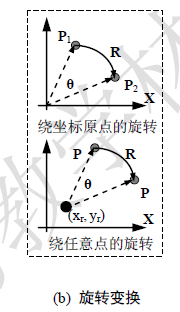
\includegraphics[width = .2\textwidth]{rotate.jpg}
    \caption{旋转}
    \label{fig:label7}
\end{figure}
要实现旋转
需指定旋转角$\theta$(绕基准点逆时针旋转时旋转角为正)
和物体旋转的旋转点(或基准点)的位
置$(x_r,y_r)$。这种变换也可描述为通过绕基准点垂直于xy 平面的旋转轴的旋转。

当基准点为坐标原点时,二维旋转变换方程为:
\begin{equation}
    \left\{
                 \begin{array}{lr}
                 x_2 = x_1\cos \theta - y_1 \sin \theta\\
                 y_2 = x_1 \sin \theta + y_1 \cos \theta 
                 \end{array}
    \right.
\end{equation}


二维旋转变换的齐次表示为:
\begin{align}
    \begin{bmatrix} x_2 & y_2& 1  \end{bmatrix} = \begin{bmatrix} x_1& y_1& 1  \end{bmatrix}
    \begin{bmatrix} 
        \cos \theta & \sin \theta & 0 \\
        -\sin\theta & \cos \theta & 0 \\ 
        0 & 0 & 1 
    \end{bmatrix}
\end{align}

当基准点为$(x_r,y_r)$时,二维旋转变换方程为:
\begin{equation}
    \left\{
                 \begin{array}{lr}
                 x_2 = x_r + (x_1 - x_r)\cos \theta - (y_1 - y_r) \sin \theta\\
                 y_2 = y_r + (x_1 - x_r) \sin \theta + (y_1 - y_r) \cos \theta 
                 \end{array}
    \right.
\end{equation}

旋转变换仍保持图形各部分间的线性关系和角度关系,变换后直线的长度不变,是
一种不变形地移动物体的刚体变换,物体上的所有点旋转相同的角度。直线段旋转是将
直线段的每个端点旋转指定的角度;多边形的旋转则是将每个顶点旋转指定的旋转角;
曲线的旋转则是旋转控制取样点。\cite{move}
\subsection{缩放变换}
\textbf{原理介绍}\par
二维比例变换改变物体的尺寸,如下图所示。
\begin{figure}[h]

    \centering
    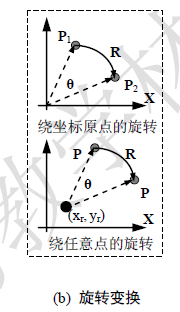
\includegraphics[width = .2\textwidth]{rotate.jpg}
    \caption{缩放}
    \label{fig:label8}
\end{figure}
相对于原点缩放时,该操作施加于多边形则可通过将
每个顶点的坐标值$(x_1,y_1)$乘以比例系数$S_x$ 和$S_y$ 以产生变换的坐标
$(x_2,y_2)$而实现:
\begin{equation}
    \left\{
                 \begin{array}{lr}
                 x_2 = x_1\cdot S_x\\
                 y_2 = y_1\cdot S_y 
                 \end{array}
    \right.
\end{equation}

比例系数$S_x$为在x方向对物体的缩放, $S_y$ 在y方向的缩放。
比例系数$S_x$和$S_y$可赋
予任何正数。小于1 缩小物体的尺寸,大于1 则放大物体。

当$S_x = S_y =1 $时,为恒等比例变换,即图形变换后不变形;

当$S_x = S_y >1 $时,图形沿两个坐标轴方向等比例放大;

当$S_x = S_y <1 $时,图形沿两个坐标轴方向等比例缩小;

当$S_x \neq S_y $时,图形沿两个坐标轴方向作非均匀的比例变换。

二维比例变换的齐次表示为:
\begin{align}
    \begin{bmatrix} x_2 & y_2& 1  \end{bmatrix} = \begin{bmatrix} x_1& y_1& 1  \end{bmatrix}
    \begin{bmatrix} 
        S_x & 0 & 0 \\
        0 & S_y & 0 \\ 
        0 & 0 & 1 
    \end{bmatrix}
    =\begin{bmatrix} x_1S_x & y_1S_y& 1  \end{bmatrix}
\end{align}

固定点缩放时,选择变换后不改变物体位置的点$(x_f,y_f)$进行缩放。顶点$(x_1,y_1)$缩放后坐标$(x_2,y_2)$为:
\begin{equation}
    \left\{
                 \begin{array}{lr}
                 x_2 = x_1\cdot S_x + x_f(1 - S_x)\\
                 y_2 = y_1\cdot S_y + y_f(1-S_Y)
                 \end{array}
    \right.
\end{equation}

用比例方程变换的物体既被缩放,又被重定位:当比例系数值大于1 时,则将被缩
放物体的坐标位置远离原点;当比例系数值小于1 时,则将被缩放物体的坐标位置拉近
原点。



多边形的缩放可将变换应用于每个顶点。而对以参数方程形式定义的其它物体的变
换则只需对方程的参数进行缩放。\cite{move}
\subsection{线段裁剪}
\subsubsection{Cohen-Sutherland算法}
\textbf{原理介绍}\par
编码算法,即Cohen-Sutherland 算法,是最早、最流行的线段裁剪算法。该算法采
用区域检查的方法,能够快速有效地判断一条线段与裁剪窗口的位置关系,对完全接受
或完全舍弃的线段无需求交,可以直接识别,大大减少求交的计算从而提高线段裁剪算
法的速度。

编码算法以图9所示的9个区域为
基础,根据每条线段的端点坐标所在的区
域,每个端点均赋以四位二进制码,称为
区域码。区域码的各位表明线段端点对于
裁剪窗口的四个相对坐标位置。
\begin{figure}[h]

    \centering
    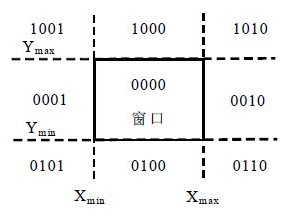
\includegraphics[width = .2\textwidth]{3-10.jpg}
    \caption{区域编码}
    \label{fig:label9}
\end{figure}
四位区域码中各位从左到右依次表示
上、下、右、左。区域码的任何位赋值为1
代表端点落在相应的区域中,否则该位为
0。若端点在裁剪窗口内,区域码为0000;
如果端点在裁剪窗口的右上角,则区域码为1010。设最左边的位为第1 位,则区域码的
生成可采用下面两种方法:

☆ 比较法

根据区域编码规则,如图9 所示,在确定区域码每位的值时,区域码各位的
值可通过将端点坐标值(x,y)与裁剪边界比较来确定:

⑴ 如果$x<x_{min}$,表示该点在裁剪窗口左边界的左边,则第1 位置1,否则置0;

⑵ 如果$x>x_{max}$,表示该点在裁剪窗口右边界的右边,则第2 位置1,否则置0;

⑶ 如果$y<y_{min}$,表示该点在裁剪窗口下边界的下边,则第3 位置1,否则置0;

⑷ 如果$x>y_{max}$,表示该点在裁剪窗口上边界的上边,则第4 位置1,否则置0。

☆ 差值法:

对可进行位操作的语言,区域码各位的值可按下列两步确定:

⑴ 计算端点坐标和裁剪边界之间的差值;

⑵ 用各差值符号来设置区域码各位的值:
第1位为$x-x{_min}$ 的符号位;第2位为
$x{_max}-x$ 的符号位;
第3位为$y-y{_min}$ 的符号位;
第4位为$y{_max}-y$ 的符号位。

判断线段是否完全在裁剪窗口内或外可采用对两个端点的区域码进行逻辑与操作的
方法,根据线段与裁剪窗口的关系可分三种情况处理:

☆ 线段完全在裁剪窗口之内

两个端点的区域码均为0000,则该线段完全在裁剪窗口之内。如图10 所示,
线段$P_5P_6$ 完全在裁剪窗口内。
\begin{figure}[h]

    \centering
    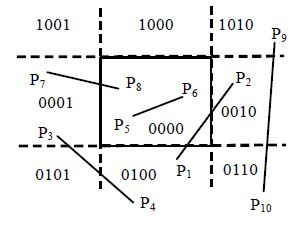
\includegraphics[width = .2\textwidth]{3-11.jpg}
    \caption{线段裁剪}
    \label{fig:label10}
\end{figure}
☆ 线段完全在裁剪窗口之外

两个端点的区域码相与后结果不为0000,则该线段完全在裁剪窗口之外。如图
10 所示,线段$P_9P_{10}$ 完全在裁剪窗口外,
$P_9$ 端点的区域码为1010,$P_10$ 端点的区域
码也为0110,与操作后结果为0010。在这种情况下,该线段可弃之。

☆ 其它

图10中$P_1P_2,P_3P_4,P_7P_8$ 都属于此类情况,需进行求交计算。
虽然$P_3P_4$ 完全落在
窗口外,但由于没有简单的判断条件,
也必须进行求交处理。求交过程为:
首先,对一
条线段的外端点与一条裁剪边界比较来确定应裁剪掉多少线段。如图10 中$P_7P_8$线段相
对裁剪窗口左边界裁剪时,根据每个端点的区域码的第一位可以确定端点的位置性质。
$P_7$ 为外端点,即落在裁剪窗口左边界的左
边,此点肯定不可见。$P_8$ 为内端点,即落在
裁剪窗口左边界的右边,为可能的可见点。
$P_7P_8$ 线段与窗口左边界求交后,可以确定应
裁剪掉的线段为$P_7$ 到$P_7P_8$ 线段与裁剪窗口
左边界的交点,而交点到$P_8$线段为剩下部
分。然后,对线段的剩下部分与其他裁剪边
界比较,直到该线段完全被舍弃或者找到位
于窗口内的一段线段为止(即线段完全可见,则不需进一步判断)。算法可按上、下、
右、左的顺序用裁剪边界检查线段的端点。在算法实现时,不必把线段与每条窗口边界
依次求交,只需按顺序检测到端点区域码的某位不为0 时,才把线段与对应的窗口边界
进行求交。

编码裁剪算法的程序流程如图11所示。\cite{move}
\begin{figure}[h]

    \centering
    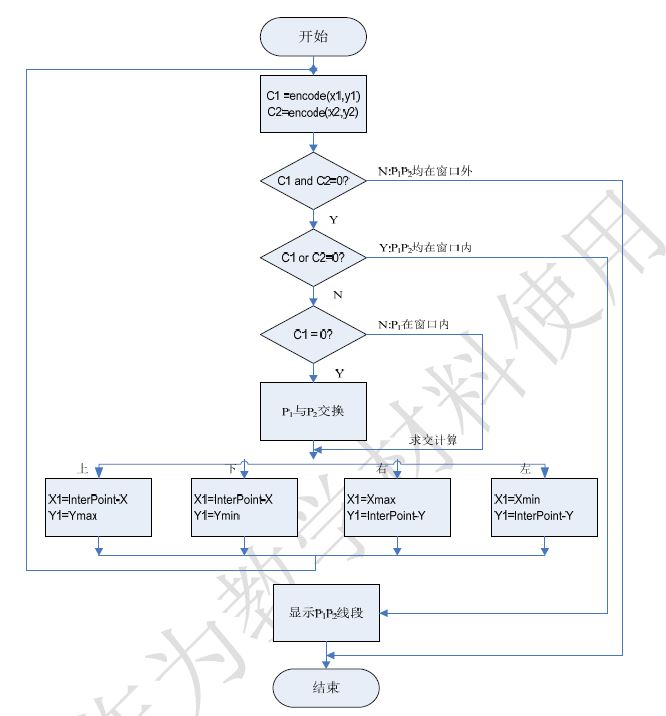
\includegraphics[width = .5\textwidth]{3-12.jpg}
    \caption{编码裁剪算法}
    \label{fig:label11}
\end{figure}
\subsubsection{Liang-Barsky算法}
\textbf{原理介绍}\par
将待裁剪线段及裁剪矩形窗口均看作点
集,那么裁剪结果即为两点集的交集。

设$P_1P_2$ 所在直线为L,记该直线(或其延长线)与裁剪窗口的两交点为
$Q_1Q_2$,称$Q_1Q_2$
为诱导窗口,它是一维的。这样,$P_1P_2$ 关于矩形窗口的裁剪结果与
$P_1P_2$ 关于诱导窗口$Q_1Q_2$ 的裁剪结果是一致的,就将二维裁剪问题化简为一维裁剪问题,如图12所
示。
\begin{figure}[h]

    \centering
    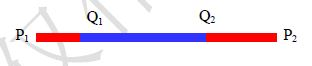
\includegraphics[width = .5\textwidth]{12.jpg}
    \caption{被裁剪直线与诱导窗口的数轴表示}
    \label{fig:label12}
\end{figure}
在一维数轴上,数轴坐标的参数表达式为:
$P=P_1+u(P_2-P_1)$。假设 $P_1$ 为数轴原点,
则 $u_{P_1}=0,u_{P_2}=1$;$Q_1Q_2$的参数分别为
$u_1$和$u_2$ ,且$u_1<u_2$;
而$ P_1P_2$和 $Q_1Q_2$间有四种位置
关系(如图13所示):
\begin{figure}[h]

    \centering
    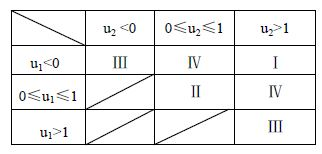
\includegraphics[width = .5\textwidth]{13.jpg}
    \caption{直线与诱导窗口关系的参数表示}
    \label{fig:label13}
\end{figure}
Ⅰ:$Q_1P_1P_2Q_2$;(完全在窗口内);

Ⅱ:$P_1Q_1Q_2P_2$;

Ⅲ:$P_1P_2Q_1Q_2$ 或$Q_1Q_2P_1P_2$ (完全在窗口外);

Ⅳ:$P_1Q_1P_2Q_2$ 或$Q_1P_1Q_2P_2$。

根据上述关系,可以得出:
$P_1P_2$ 至少部分可见的充要条件为:
$max(u_{P_1},u_1) \leq min(u_{P_2},u_2)$;

且其可见部分的区间为:
$[max(u_{P_1},u_1),min(u_{P_2},u_2)]$。

转化为一维问题后,为解决二维裁剪问题,只要生成诱导窗口。
图12中,$P_1P_2$
所在直线 Line 与窗口左、右、上、下四边界所在直线交点分别为L、R、T 和B;$Q_1Q_2$
为诱导窗口;
记窗口左右边界所在直线夹成的带形区域为$A_1$;
窗口上下边界所在直线夹
成的带形区域为$A_2$;窗口区域为Window。那么,诱导窗口Q1Q2 计算可如下:

\begin{align}
    Q_1Q_2= Line \cap Window=Line \cap (A_1 \cap A_2)= (Line \cap A_1) \cap (Line \cap A_2)=LR \cap TB
\end{align}

其中:LR 和TB 分别为在水平方向和垂直方向的参数区间。上式给出了$Q_1Q_2$ 对应的参数
区间,如图14(b)所示。
\begin{figure}[h]

    \centering
    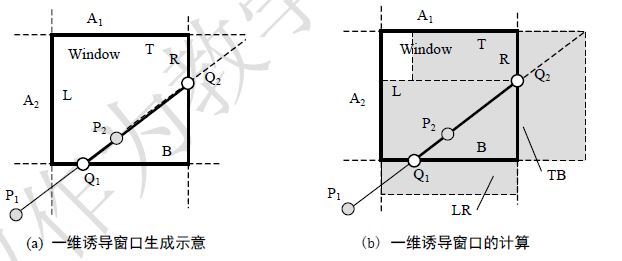
\includegraphics[width = .5\textwidth]{14.jpg}
    \caption{诱导窗口的生成和计算}
    \label{fig:label14}
\end{figure}
这样,$P_1P_2$ 的可见部分VW可计算为:
\begin{align}
    VW= P_1P_2 \cap Q_1Q_2=P_1P_2 \cap LR \cap TB
\end{align}

参数化形式的裁剪条件:
\begin{equation}
    \left\{
                 \begin{array}{lr}
                 xw_{min} \leq x_1 + u \cdot \Delta x \leq xw_{max}\\
                 yw_{min} \leq y_1 + u \cdot \Delta y \leq yw_{max} 
                 \end{array}
    \right.
\end{equation}

可统一表示为:$u \cdot p_k \leq q_k$。其中,k=1,2,3,4,对应裁剪窗口的左、右、上、下边
界;参数p、q 定义为:
\begin{equation}
    \left\{
                 \begin{array}{lr}
                 p_1 = \Delta x,q_1 = x_1 - xw_{min}\\
                 p_2 = \Delta x,q_2 = xw_max - x_1\\
                 p_3 = \Delta y,q_3 = y_1 - yw_{min}\\
                 p_4 = \Delta y,q_4 = yw_{max} - y1 
                 \end{array}
    \right.
\end{equation}

根据$p_k$可以确定线段与裁剪窗口的相互位置关系:

① 若$p_k=0$,直线平行于裁剪边界之一。此时,如果同时满足$q_k<0$,则线段完全在
边界外;如果同时满足$q_k \geq 0$,线段平行于裁剪边界,并且在窗口内;

② 当$p_k<0$, 线段从裁剪边界延长线的外部延伸到内部;

③ 当$p_k>0$,线段从裁剪边界延长线的内部延伸到外部。

因而,当$p_k$非零时,可计算出线段与边界k 或延长线交点的u 值:
$u=q_k/p_k$;
对每条线段,可计算出参数$u_1$和$u_2$,它们定义了在裁剪矩形内的线段部分:
如果$u1>u2$,则线段完全落在裁剪窗口外,被舍弃;否则,被裁剪线段的端点由参数u 的两个值
计算出来:u1 的值由线段从外到内遇到的矩形边界所决定(p<0),对这些边界计算参数:
$r_k=q_k/p_k$,$u_1$取0和各个$r_k$值之中的最大值;
$u_2$ 的值由线段从内到外遇到的矩形边界所决
定(p>0),对这些边界计算参数:$r_k=q_k/p_k$,$u_2$ 取1和各个$r_k$值之中的最小值。

在具体实现时,算法的实现过程如下:

(1) 将线段交点的参数初始化为 $u_1=0,u_2=1$;

(2) 定义一个函数,用 p、q 来判断是舍弃线段还是改变交点的参数r:

    当p<0 时,参数r 用于更新$u_1$;

    当p>0 时,参数r 用于更新$u_2$:

    如果更新$u_1$ 或$u_2$ 后使$u_1>u_2$,则舍弃该线段;

    否则,更新适当的u 值仅仅求出了交点,缩短线段。

(3) p、q 的四个值经过测试后,当p=0 且q<0 时,说明该线段平行于边界且位于边
界之外,舍弃该线段。假如该线段未被舍弃,
则裁剪线段的端点由$u_1、u_2$ 值决定。

(4) 反复调用该函数,计算出各个裁剪边界的p、q 值,进行判断。\cite{move}

\textbf{对比分析}\par
通常,梁友栋-Barsky 算法比Cohen-Sutherland 算法更有效,因为需要计算的交点数
目减少了,更新参数$u_1、u_2$ 仅仅需要一次除法;线段与窗口的交点仅需计算一次就能得
出$u_1、u_2$ 的最后值;相比之下,即使一条线段完全落在裁剪窗口之外,Cohen-Sutherland
算法也要对它反复求交点,而且每次求交计算都需要除和乘。梁友栋-Barsky 和Cohen-
Sutherland 算法都可以扩展为三维裁剪算法。\cite{move}

\section{系统介绍}
\subsection{核心算法模块}
目前为止,在助教提供的系统框架基础上,运用前文中的算法完成了cg\_algorithms.py中直线,多边形和椭圆的生成,以及平移、旋转、缩放等图元的变换操作。
\subsection{命令行界面(CLI)程序}
\subsubsection{数据结构}
画布可以用一个矩阵canvas表示。创建的图元用item\_dict这一字典结构存储,键为图元id,
值为一个list,其中存储图元的类型,给定点,实现所用算法和颜色。
color用一个三元uint8数组表示,分别对应RGB的值。

\subsubsection{设计思路}
先获取指令文件,对于每一行用空格分隔的指令,采用split转换为一个list,逐个解析,对于第一个元素也就是指令类型,分别有不同的处理方法,如下:
另外关于图元变换的指令,起初我想读到相应命令就绘制新的图元,但这样很不方便,就记下要变换的图元和变换参数,等待savecanvas时一起绘制。
\begin{itemize}
  \item [·]
  重置画布

  借助于助教的框架,画布可以用一个矩阵表示,矩阵的每个元素是图像的一个像素。重置即为清除所有图元,item\_dict为空。
  
  \item [·]
  保存画布
  
  遍历图元,根据图元类型选择相应的函数生成对应的点,再对这些点进行着色。若类型是图元变换相关,则找到原来的图形再使用图元变换函数,形成新的着色点。
  采用Image.fromarray实现从array到image的转换,再用save方法保存到指定路径。

  \item [·]
  设置画笔颜色

  根据输入设置color的值。

  \item [·]
  绘制线段

  依据指令格式,依次截取图元id,起止坐标,算法,类型为line,加入item\_dict。

  \item [·]
  绘制多边形

  依据指令格式,依次截取图元id,坐标列表,算法,类型为polygon,加入item\_dict。
  
  \item [·]
  绘制椭圆(中点圆生成算法)
  
  依据指令格式,依次截取图元id,坐标列表,算法默认为中点圆,类型为polygon,加入item\_dict。

  \item [·]
  绘制曲线
  
  \item [·]
  图元平移

  依据指令格式,依次截取图元id,dx,dy,修改图元
  id为旧id加上translate标志,类型为命令行参数加上旧图元id,其他属性照旧,加入item\_dict。
  
  \item [·]
  图元旋转

  依据指令格式,依次截取图元id,dx,dy,修改图元
  id为旧id加上rotate标志,类型为命令行参数加上旧图元id,其他属性照旧,加入item\_dict。
  
  \item [·]
  图元缩放

  依据指令格式,依次截取图元id,dx,dy,修改图元
  id为旧id加上scale标志,类型为命令行参数加上旧图元id,其他属性照旧,加入item\_dict。

  \item [·]
  对线段裁剪
  
\end{itemize}
\section{总结}
目前,我学习了一些图形绘制的算法并用python语言实现了一部分。对于图形学的学习,我还刚刚开始,学习了一些经典算法,正在充实自己的理论,尝试着运用到实践之中。
我完成了大部分命令行界面程序,并在实现过程中发现了之前算法模块的一些bug:
\begin{itemize}
    \item [1)]
    在rotate中,命令给出的参数单位是角度,而math中三角函数的参数是弧度,需要进行相应转换。
    \item [2)]
    在一些指令对应的处理函数中,有相似的部分,我起初复制黏贴,有很多细节疏忽了,事后还要慢慢修改。
    \item [3)]
    在生成线段时,从y0
    循环到y1,需要考虑两者的大小关系。
\end{itemize}

\bibliographystyle{plain}%
%"xxx" should be your citing file's name.
\bibliography{ref}


%\bibliography{info}
%\bibliographystyle{plainnat}

\end{document}
/*进度报告/系统报告要求
•	在上个月报告的基础上添加本月新的内容即可,无需从头重写
•	报告内容包括:
o	已完成或拟采用算法的原理介绍、自己的理解、对比分析等
o	已完成或拟采用的系统框架、交互逻辑、设计思路等
o	介绍自己系统中的巧妙的设计、额外的功能、易用的交互、优雅的代码、好看的界面等(可选)
•	请附上联系方式(邮箱或QQ等),以便出现问题时及时联系
•	需注明在实现作业过程中使用的参考资料,包括技术博客等
•	可添加附加材料(觉得需要附加说明的代码等)*/